\section{UserOption}
\label{sec:userOption}

\begin{figure}[h!] 
	\centering
	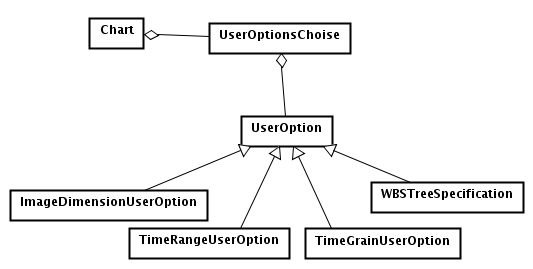
\includegraphics[width=0.7\textwidth]{../Milestone1-DomainModel/img/UserOptionDetail.png}
	\caption{UserOptions and choice}
	\label{fig:userOption} 
\end{figure}

Quando un generico client (potrebbe essere sia una persona fisica che un
oggetto astratto) della nostra implementazione della specifica vuole generare
un \emph{Chart} pu\`o guidare la generazione decidendo alcuni fattori che sono
di suo interesse. Questi fattori vengono modellati dal concetto di
\emph{UserOption}.

Ogni \emph{Chart} espone una lista di \emph{UserOption} per dare al client la
possibilit\`a di esprimere quali informazioni guidare. Questa lista varia da
\emph{Chart} a \emph{Chart}\footnote{creare un reference dove vengono mappate
questa relazione: potrebbe essere un appendici di questo documento??}.

Il concetto di lista di \emph{UserOption} \`e catturato in
\emph{UserOptionsChoice}.

Procediamo per passi: nelle prossime subsection osserviamo due aspetti che
trattarli insieme potrebbe non essere sufficiente per esporli in modo chiaro.

\subsection{\emph{UserOption}'s Instances}
\label{subsec:UserOptionInstances}
Questa \`e stata una decisione non molto facile da prendere. Il problema \`e
questo: nella specifica abbiamo che per ogni \emph{Chart} il committente ha
dichiarato quali \emph{UserOption} mostrare. Queste per\`o non rappresentano un
concetto che vogliamo catturare nel nostro modello, ma allo stesso tempo sono
\emph{istanze} (un insieme discreto quindi) di elementi che fissa il
committente.

Per questo motivo decidiamo di codificare questo insieme discreto in questo
documento e la successiva enumerazione \`e da considerarsi parte integrante del
diagramma inserito come figura.

Rappresentiamo il concetto espresso sopra indicando due descrizioni con questa
struttura di codifica:
\begin{itemize}
  \item \emph{istanze}, dove inseriamo tutte le possibili \emph{UserOption} che
  non possono essere ancora raffinate
  \item \emph{specializzazioni} dove inseriamo tutte le possibili
  specializzazioni di \emph{UserOption} che possono essere ancora raffinate,
  ripetendo in modo ricorsivo questa struttura di codifica
\end{itemize}

Le successive descrizioni sono relative al concetto di \emph{UserOption}:
\begin{description}
  \item[istanze]\quad
  \begin{description}
	\item[TaskNameUserOption] genera una stringa contenente il nome del task.
	Questa stringa si pu\`o usare, per esempio, per appenderla alla
	rappresentazione dell'identificatore del task definito nel \emph{project plan}
	\\ \emph{Dominio di valorizzazione = boolean}
	\item[EffortInformationUserOption] crea un stringa da inserire sulla destra
	della reppresentazione \emph{GanttTaskbox}. la stringa viene costruita in modo
	diverso in base al task (solo coppia di interi per task composti, mentre per
	task atomici vengono aggiunte i dettagli di ogni risorsa assegnata, vedi
	sezione 1, punto 2, pag 2 del documento di specifica)
	\\ \emph{Dominio di valorizzazione = boolean}
	\item[PlannedDataUserOption] definisce la tripla \emph{(duration, effort,
	cost)} per planned info.
	\\ \emph{Dominio di valorizzazione = boolean}
	\item[PlannedTimeFrameUserOption] definisce la coppia \emph{(start date, end
	date)} per planned info.
	\\ \emph{Dominio di valorizzazione = boolean}
	\item[ResourcesUserOption] definisce la tripla \emph{(effort, person, role)}
	\\ \emph{Dominio di valorizzazione = boolean}
	\item[ActualTimeFrameUserOption] definisce la coppia \emph{(start date, end
	date)} per actual info.
	\\ \emph{Dominio di valorizzazione = boolean}
	\item[ActualDataUserOption] definisce la tripla \emph{(duration, effort,
	cost)} per actual info (questa opzione include anche la \emph{completition
	bar}).
	\\ \emph{Dominio di valorizzazione = boolean}
	\item[AlertMarkUserOption] notifica quando ci sono delle differenze fra le
	informazioni planned e quelle actual
	$$good_{news} \rightarrow
 \Delta$$$$bad_{news} \rightarrow \Delta!$$ $a \rightarrow b$ rappresenta che
 $a$ viene rappresentato con il simbolo $b$
 	\\ \emph{Dominio di valorizzazione = boolean}
	\item[ReplicateArrowUserOption] nei punti in cui due freccie (rappresentanti
	ciascuna una dipendenza) convergono verso un punto di incontro per
 entrare nel task \emph{dipendente} (deve essere usato un punto di incontro nel
 caso di dipendenze per un task perch\`e \`e un requisito del committente: in
 ogni task entra \emph{al pi\`u} una freccia) 
 	\\ \emph{Dominio di valorizzazione = boolean}
 	\item[UseDifferentPatternForCrossingLinesUserOption] se due linee
 	rappresentanti una dipendenza di sovrappongono, allora \`e utile disegnarle
 	in modo diverso\footnote{non \`e ben specificato se rispetto al colore
 	(opzione non molto fattibile per la stampa su carta perch\`e si utilizza la
 	scala di grigi) oppure con pattern diversi (dotted, broken\ldots)} \`E
 	richiesto di distinguere coppie di linee che si sovrappongono, questo quindi
 	non vincola ad usare n pattern per ogni coppia di sovrapposizione: possiamo
 	ripetere il pattern per altre coppie che si sovrappongono, ma la cui
 	sovrapposizione non \`e con coppie che utilizzano lo stesso pattern per
 	distinguersi.
 	\\ \emph{Dominio di valorizzazione = boolean}
 	\item[TimeGapsUserOption] viene mostrata sopra la linea che rappresenta
 	la dipendenza, la differenza tra le date di fine \emph{needed} task e inizio
 	\emph{dependent} task.
 	\\ \emph{Dominio di valorizzazione = boolean}
 	\item[CriticalPathUserOption] calcolare e rappresentare i percorsi critici
 	\\ \emph{Dominio di valorizzazione = boolean}
 	\item[MaxCriticalPathNumberUserOption] indica il numero massimo di critical
 	path che si vogliono calcolare e visualizzare
 	\\ \emph{Dominio di valorizzazione = integer}
 	\item[OpenInNewWindowUserOption] apre la rappresentazione del \emph{Chart} in
 	una nuova finestra diversa da quella dove si \`e richiesta la generazione.
 	\\ \emph{Dominio di valorizzazione = boolean}
  \end{description}

  \item[specializzazioni] \quad
  \begin{description}
    \item[WBSTreeSpecification] rappresenta il livello di dettaglio scelto per
    la rappresentazione nel \emph{Chart}:
	    \begin{description}
	  		\item[istanze] \quad
	  		\begin{description}
				\item[LevelSpecificationUserOption] viene esploso il \emph{project plan}
				al livello $l$ specificato
				\\ \emph{Dominio di valorizzazione = integer}
				\item[UserCustomSpecificationUserOption] viene rappresentato il
				\emph{project plan} come selezionato nei tab \emph{(planned $\mid$ actual)
				View}
				\\ \emph{Dominio di valorizzazione = user interactive input}
		  	\end{description}
	  	\end{description}

	\item[ShowDependenciesUserOption] rappresenta nel \emph{Chart} alcuni
	tipi di dipendenze. Quelle disponibili sono:
	    \begin{description}
		  \item[istanze] \quad
		  \begin{description}
			\item[FinishToStartDependenciesUserOption] mostra la relazione di
			\emph{finish to start} fra coppie di task
			\\ \emph{Dominio di valorizzazione = boolean}
			\item[CompositionDependenciesUserOption] mostra la relazione di
			\emph{composition} fra coppie di task
			\\ \emph{Dominio di valorizzazione = boolean}
			\item[ShowCompleteDiagramDependencies] mostra la relazione di \emph{finish
			to start} rispetto alle milestone \emph{start, end} project, per i
			tasks che non sono necessari oppure dipendono da altri tasks.
			\\ \emph{Dominio di valorizzazione = boolean} 
		  \end{description}
		 
		\end{description}

	\item[TimeGrainUserOption] indica la grana temporale con cui identificare i
	passi verticali del \emph{GanttChart}:
	    \begin{description}
		  \item[istanze]\quad
		  \begin{description}
			\item[HourlyGrainUserOption] \emph{Dominio di valorizzazione = boolean}
			\item[DailyGrainUserOption] \emph{Dominio di valorizzazione = boolean}
			\item[WeaklyGrainUserOption] \emph{Dominio di valorizzazione = boolean}
			\item[MonthlyGrainUserOption] \emph{Dominio di valorizzazione = boolean}
			\item[AnnuallyGrainUserOption] \emph{Dominio di valorizzazione = boolean}
		  \end{description}
		\end{description}

	\item[ImageDimensionUserOption] rappresenta la dimensione dell'immagine che
	\`e possibile rappresentare:
	    \begin{description}
	  	\item[istanze]\quad
		  \begin{description}
			\item[CustomDimUserOption] \emph{Dominio di valorizzazione = integer
			$\times$ integer}
			\item[FitInWindowDimUserOption] \emph{Dominio di valorizzazione = boolean}
			\item[OptiomalDimUserOption] \emph{Dominio di valorizzazione = boolean}
			\item[DefaultDimUserOption] \emph{Dominio di valorizzazione = boolean}
		  \end{description}
	\end{description}
	
	\item[TimeRangeUserOption] indica il range temporale che si vuole
	rappresentare nel \emph{GanttChart}:
	    \begin{description}
	  		\item[istanze]\quad
			  \begin{description}
				\item[CustomRangeUserOption] \emph{Dominio di valorizzazione = date
				$\times$ date}
				\item[WholeProjectRangeUserOption] \emph{Dominio di valorizzazione = boolean}
				\item[FromStartRangeUserOption] \emph{Dominio di valorizzazione = date}
				\item[ToEndRangeUserOption] \emph{Dominio di valorizzazione = date}
			  \end{description}
		\end{description}

  \end{description}
\end{description}

\subsection{\emph{UserOptionsChoice}}
Questo concetto \`e, secondo la nostra analisi, molto importante in quanto ci
permette di astrarre dal client che richiede una generazione.

Il motivo per cui abbiamo introdotto questo concetto \`e di poter lavorare lato
server usando \emph{UserOptionsChoice} per controllare quali informazioni il
client vuole guidare. In questo modo non siamo vincolati ad accedere ai dati
inviati per \emph{POST, GET} dalla form HTML, ma possiamo direttamente guardare
in \emph{UserOptionsChoice}. Queste ci permette di disaccopiare il processo di
generazione della maschera di input di una pagina HTML. 

Se vogliamo utilizzare il processo di generazione (che comunque \`e
server side) scrivendo un programma client (GUI o da riga di comando) che
costruisce una HTML request ad hoc (dovremo definire una grammatica e
attribuire la semantica ai contesti, questo \`e necessario, non ch\`e scrivere 
un parser), usando \emph{UserOptionsChoice} e il suo disaccoppiamento ci sar\`a
possibile farlo. 

Una volta ricevuta la response possiamo maneggiare la pagina
inviata come una response HTML valida e usarla per i nostri obiettivi (possiamo
rihiedere l'immagina generata, o il file PDF generato, salvandolo in
locale, oppure visualizzando lo stesso con un browser, ma possiamo anche
inserire in un db oppure farci dei test sopra\ldots).

Dovremo quindi costruire un oggetto che si incarica di costruire
\emph{UserOptionsChoice} in base al tipo di richiesta ricevuta (da una pagina
html come \`e il caso di PMango, oppure una richiesta da un client indipendente
scritto in un qualche linguaggio). Una volta costruito l'insieme delle
\emph{UserOption} \`e possibile iniziare la generazione. Questo sar\`a delegato
alla fase di progettazione.
